\documentclass[12pt]{jsarticle}
\usepackage[dvipdfmx]{graphicx}
\usepackage{amsmath}
\usepackage{array}

\title{最急降下法}
\author{大枝 真一}
\date{}

\begin{document}
\maketitle

\section{はじめに}
機械学習では,なんらかの数理モデルを仮定する.このときに,目的関数(誤差関数)を設定して,この関数の
最小値(or 最大値)求める必要がある.この関数が解析的に陽に解けるときは問題ないが,一般的に機械学習
で扱う目的関数は非常に複雑であるため,解析的に陽に解けないことがほとんどである.あるいは,人間が時間
をかけて解析的に解いて厳密解を得るよりも,計算機を用いて近似値を短時間で求める方が有益なことが多い.
このような繰り返しの計算で代表的な手法が最急降下法である.

\section{最急降下法}
ここでは,最急降下法の説明のため,式(\ref{eq:easy})に示す目的関数の最小値を求めることを考える.

\begin{equation}
  f(x)=(x-2)^2 + 1
  \label{eq:easy}
\end{equation}

関数を図に示すと図\ref{fig:easy}のようになる.

図\ref{fig:easy}からわかるように,この関数はx=2のときに最小値をとる.今は,最小値の値にはとくに関心がなく,xがいくらのとき最小値をとるかを知り
たい.このような目的関数への入力xはパラメータと呼ぶ.一般的な機械学習では事前に設定した目的関数を最
小にするパラメータを,観測したデータから求めることになる.

\begin{figure}[ht]
  \begin{center}
    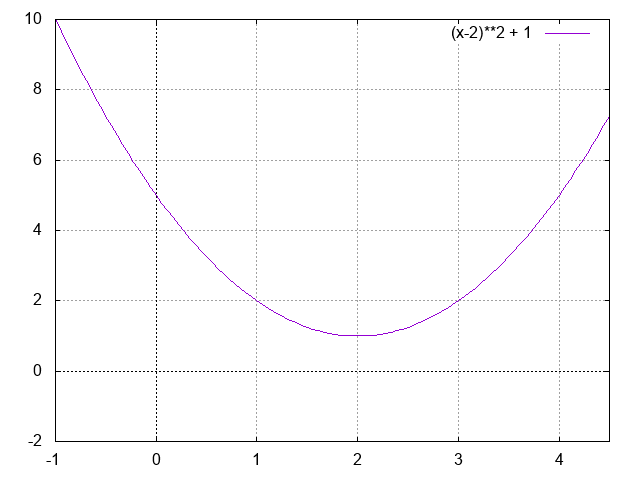
\includegraphics[scale=0.6]{fig/easy.png}
  \end{center}
  \caption{求めたい目的関数}
  \label{fig:easy}
\end{figure}

\subsection{解析的に解く}
関数の最小値を求めるには,関数の凸性を調べた後,微分して0になる点を探す.

式(\ref{eq:easy})を微分すると式(\ref{eq:easy-dash})のようになる.
\begin{equation}
  f'(x)=2(x-2)
  \label{eq:easy-dash}
\end{equation}

これが0になるとき,関数の傾きが0であることがわかるので,式(\ref{eq:easy})は関数の形状より,下に凸で
最小値を1つしか持たないことがわかるので,$f'(x)=2(x-2)=0$より,$x=2$のとき最小値をとる.

\subsection{最急降下法で解く}
最急降下法は,関数$f(x)$の傾きから繰り返し$x$を更新し,最小値(厳密には極小値)を求める反復法である.

最急降下法の更新は以下の式で行う.
	
\begin{equation}
  x_{t+1} = x_{t} - \eta \frac{\partial f(x_{t})}{\partial x_{t}}
  \label{eq:gdm}
\end{equation}
	
$\eta$は学習係数で$\eta = 0.01$など小さい値をあらかじめ決めておく.$\eta$を大きくするほど学習速度は
向上するが大きすぎると収束せず振動や発散をしてしまう.逆に小さいほど,学習は安定して収束するが学習速度が
低下してしまう.したがって,$\eta$は適切な値の設定が必要となる.

最初に適当に$x$の初期値を決める.初期値から偏微分$\frac{\partial f(x)}{\partial x}$を求め,式
(\ref{eq:gdm})に代入し,$x$を更新する.このとき,$x$が極小値のときよりも大きければ傾きは
$\frac{\partial f(x)}{\partial x} > 0$となるため,$x$は小さくなり,$f(x)$は極小値に近づく.それに対
して,$x$が極小値のときよりも小さければ傾きは$\frac{\partial f(x)}{\partial x} < 0$となるため,$x$は
大きくなり,$f(x)$はやはり極小値に近づく.このように$x$がどちらの場合でも更新後$f(x)$は極小値に近づ
く.また,傾きは極小値に近づくほどゆるやかになるため,修正量も小さくなり,$\eta$が適切な値の場合は,
振動をせずに収束に向かう.このように最急降下法では,着実に極小値には近づくが,関数の形状や初期値によっ
ては,最小値を求めることができない場合がある.

\subsection{実際に最急降下法で解いてみる}
初期値3.0,学習係数0.1として,最急降下法で
式(\ref{eq:easy})の関数の最小値を求めてみよう.式(\ref{eq:easy})を微分すると式(\ref{eq:easy-dash})と
なるので,更新式は以下のようになる.

\begin{align*}
  x_{t+1} &= x_{t} - \eta \frac{\partial f(x_{t})}{\partial x_{t}} \\
  &= x_t - 0.1\times 2(x_t-2)
\end{align*}
\label{eq:gdm2}

更新式が求まったので,$x_0=3.0$として,$x_t$を繰り返し求めてみよう.
\begin{align*}
  x_0 &= 3.0 \\
  x_1 &= 3.0 - 0.1\times 2(3.0-2) \\
      &= 3.0 - 0.2 \\
      &= 2.8 \\
  x_2 &= 2.8 - 0.1\times 2(2.8-2) \\
      &= 2.8 - 0.16 \\
      &= 2.64 \\
  x_3 &= 2.64 - 0.1\times 2(2.64-2) \\
      &= 2.64 - 0.128 \\
      &= 2.512 \\
\end{align*}

このように,繰り返していくと,徐々に最小値をとるパラメータ$x=2$に近づいていく.

\end{document}
